% Experimental evaluation of output-guided behavioral decomposition, as implemented in ace/.
%
% Drop-in results section. Companion to reports/METHODOLOGY.tex and written to the same
% rules: every number below comes from a recorded run, and the artifact it came from is named
% in a comment so the two can be checked against each other.
%
% Requires the macros \ACE, \Tr, \Grammar, \Regions already used by the methodology section,
% and the packages booktabs and pgfplots in addition to the ones the
% paper already loads (amsmath, algorithm, algorithmicx, tikz). Delete the
% \section line below if the surrounding paper already opens the section.
%
% Sources, all regenerable:
%   results/recovery_summary.json      RQ2   tools/score_recovery.py, declared only
%   results/sweeps/budget.jsonl        RQ3   tools/sweep.py --budgets ... --seeds 10
%   results/sweeps/grammar.jsonl       RQ4   tools/sweep.py --grammars G1,...,G5
%   results/sweeps/cost.jsonl          RQ5   tools/sweep.py --jobs 1
%   results/sweeps/baseline.jsonl      RQ1   tools/baseline.py
% Table bodies are printed by tools/report_rqs.py; nothing here was transcribed by hand.

\section{Experimental Evaluation}
\label{sec:results}

\subsection{Setup}
\label{sec:setup}
The benchmark is eleven RTL blocks in three families: three sub-blocks of the Ibex RISC-V
core (\texttt{ibex\_alu}, \texttt{ibex\_csr}, \texttt{ibex\_multdiv\_fast}), three protocol
blocks written for this benchmark (\texttt{apb\_slave}, \texttt{arbiter4},
\texttt{fifo\_sync}), and five arithmetic blocks. Each design is driven by a SystemVerilog
testbench through a planned set of scenarios and writes one row per cycle over the
\emph{observable interface only} --- no clock, no internal state --- so every result below is
obtained from what a black-box user of the IP can see. Each design contributes five mining
runs, three independently seeded held-out runs used only in Step~5, and two stress runs whose
environment violates the contracts' assumptions and which are never mined.
\texttt{accumulator} and \texttt{sqrt} carry ten mining and six held-out runs. Table~\ref{tab:setup}
gives the corpus and the size of the hand-encoded reference set each design is scored against.

One vocabulary is used throughout. \ACE{} is given the design's \texttt{extra\_props},
which for this benchmark were written from the reference contracts, together with the
propositions it reads off each region: conjunctions over distinct signals, relations between
two signals, sign splits, same-stem sums and signal transitions, each kept only where the
traces exhibit it.\footnote{\texttt{ace/vocabulary.py}, declared by
\texttt{ace/mining.py:\_vocabulary}.} What a hint-based miner's vocabulary can express is a
question about the miner; this evaluation is about the decomposition, so the vocabulary is
held fixed across every comparison below and recall measures the flow rather than the
vocabulary. HARM is the only temporal backend; a run on a machine without it exits non-zero
and writes nothing, so every number reported here came from the same
miner.\footnote{\texttt{ace/backends.py:92--105}.}

All comparisons between clauses --- equivalence, refinement, subsumption --- are decided by
\ACE{}'s own evaluator over the observed corpus.\footnote{\texttt{ace/validation.py:80--137},
\texttt{343--365}.} They are statements about agreement on the traces at hand, not proofs.
A reference clause is scored \emph{equivalent} when a mined clause says exactly it,
\emph{mined-stronger} when a mined clause implies it (a refinement, and an acceptable
recovery), \emph{mined-weaker} when only a weaker form came back, and \emph{missed}
otherwise --- which folds in the case where every mined clause is incomparable to it.
\emph{Exact} recall is the equivalent share; \emph{acceptable} recall counts equivalent plus
refinements.

\begin{table}[t]
\centering
\caption{The benchmark. \emph{in}/\emph{out} are interface signals, \emph{ev} the declared
output events, \emph{A}/\emph{G} the hand-encoded reference assumptions and guarantees.}
\label{tab:setup}
\begin{tabular}{llrrrrrrr}
\toprule
design & family & in & out & ev & runs & samples & A & G \\
\midrule
% tools/report_rqs.py --section setup
ibex\_alu & Ibex & 3 & 3 & 3 & 5 & 6000 & 2 & 18 \\
ibex\_csr & Ibex & 3 & 2 & 2 & 5 & 2500 & 2 & 4 \\
ibex\_multdiv\_fast & Ibex & 6 & 2 & 1 & 5 & 7500 & 4 & 13 \\
apb\_slave & protocol & 6 & 3 & 2 & 5 & 6000 & 4 & 18 \\
arbiter4 & protocol & 5 & 6 & 2 & 5 & 5000 & 2 & 18 \\
fifo\_sync & protocol & 4 & 4 & 2 & 5 & 6000 & 2 & 18 \\
accumulator & arithmetic & 3 & 2 & 1 & 10 & 19000 & 3 & 5 \\
adder\_8bit & arithmetic & 3 & 2 & 1 & 5 & 2500 & 2 & 7 \\
comparator\_3bit & arithmetic & 2 & 3 & 3 & 5 & 2000 & 1 & 8 \\
multi\_16bit & arithmetic & 4 & 2 & 1 & 5 & 5000 & 3 & 8 \\
sqrt & arithmetic & 3 & 3 & 2 & 10 & 20000 & 3 & 13 \\
\midrule
total & & & & 20 & 65 & 81500 & 28 & 130 \\
\bottomrule
\end{tabular}
\end{table}

\subsection{RQ1: what decomposition covers, and what it reaches}
\label{sec:rq1}
Decomposition is not an optimisation the flow may skip. A contract's $A$ is an environment
invariant \emph{conditioned on a region's trigger}: the same invariant computed over the whole
corpus is a global range, and it is the conditioning that turns it into an assumption. Without
a region there is nothing to condition on, so undecomposed mining can state only what is true
everywhere. This section reports three quantities: how much of each design's assumption side
each approach covers, how much of its guarantee side, and how many obligations the flow
reaches that undecomposed mining cannot express at all.

Direct mining is used as a \emph{control} rather than a competitor. It is built from the flow's
own parts with Steps~1--3 removed: HARM is pointed at the full mining corpus instead of at
extracted episodes, with the same grammar, the same vocabulary, the same horizon and the same
reset, and its output is scored by the same
comparison.\footnote{\texttt{tools/baseline.py}, reusing \texttt{ace/\_\_main\_\_.corpus\_traces}
and \texttt{ace/mining.\_mine\_temporal}.} Run boundaries are preserved on both sides --- the
corpus is passed as one CSV per run --- so the only thing that differs is whether the miner
sees whole executions or clipped episodes. Because a contract's $A$ is a conjunction of
propositional invariants and a temporal miner emits implications, the control is also given the
flow's invariant miner over the whole corpus; without it the control would return no assumption
at all, for a reason that has nothing to do with decomposition. On both sides the assumption
side is scored against each mined invariant and against the conjunction of all of
them.\footnote{\texttt{tools/score\_recovery.py}, \texttt{conjunction}.}

\emph{Assumptions.} The \emph{A} columns of Table~\ref{tab:rq1} are where the two differ most:
acceptable recall on the assumption side is 83\% for the flow against 40\% for the control,
ahead on eight designs and behind on none. On \texttt{ibex\_multdiv\_fast}, \texttt{arbiter4}
and \texttt{sqrt} the control reads \emph{zero} where the flow reads 75\%, 100\% and 67\%. Zero
does not mean it mined nothing --- it mines 16, 15 and 7 invariants on those designs and
relates to every reference assumption --- but not one of its matches is equivalent to a
reference or stronger than it. What it produces are global ranges: \texttt{data\_in <= 255}
where the reference asks for \texttt{rst\_n == 1}. The mechanism is the one the methodology
describes: an invariant computed over the whole corpus is a bound, while the same invariant
computed at the anchors of a region and conditioned on the trigger is an environment
restriction. One qualification belongs with this number rather than after it. Of the flow's 22
assumption recoveries that are equivalent or stronger, 13 come from the guard search of
\texttt{mining.refine}, seven from region-scoped invariants and two from the conjunction
candidate; \texttt{refine} has no counterpart on the control side, so the comparison is not
like-for-like. It is also not separable from decomposition, since there is no region to search
guards over without it.

\emph{Guarantees.} Counted as reference clauses for which any related clause came back, the two
are level: 118 of 130 for the control against 117 of 130 for the flow, and per design the
\emph{G} columns differ by at most two clauses either way. Episode extraction does not hide
behavior from the miner. Where the two differ in \emph{form} rather than in coverage, it is
usually because the flow states the obligation more tightly: of the 28 references the control
matches exactly and the flow does not, 23 come back from the flow as clauses that \emph{imply}
the reference, and only two are lost outright. On \texttt{accumulator} the reference
$G(\mathit{rst\_n}=0 \mid\rightarrow \mathit{valid\_out}=0)$ returns as
$G(\mathit{valid\_in}=0 \wedge \mathit{data\_out}=0 \mid\rightarrow \mathit{valid\_out}=0
\wedge \mathit{data\_out}=0)$, a stronger statement about the same behavior; the control is
handed the identical vocabulary but has no region to condition on, so its antecedents stay
broad and land on the documented text itself. Ten references are genuinely lost to the flow:
four it proposed and then discarded as violated or vacuous on the region they were mined from,
and six were never proposed.

\emph{Region-specific guarantees, where the flow has the edge.} The reference set cannot show
the rest, because every reference was validated to hold over the whole corpus and so lies
within the control's reach by construction.\footnote{\texttt{benchmarks/run.py --validate-only};
per-clause evidence in \texttt{benchmarks/traces/<design>/reference\_check.json}.} Clipping to
episodes removes falsifying positions, so more clauses hold on an episode set than on the whole
corpus, and 2405 of the flow's 14911 kept guarantees are region-specific: violated by the
corpus outside the region they were mined from. The control cannot emit those, and not because
it ranks them low. It has no assumptions --- it emits what holds on whole traces --- and a
template gives it one antecedent slot filled by one declared
proposition,\footnote{\texttt{ace/backends.py:GRAMMARS}; the decision-tree placeholder that
would build a conjunction is only in \texttt{G5}, which no design runs (\S\ref{sec:rq4}).} so
the region's condition would have to be in its vocabulary already, conjoined with the
antecedent it needs. The flow never pays that price: it obtains the condition by restricting
which samples the miner sees. Asking how often that matters --- whether any declared
proposition makes the same consequent globally true \emph{while covering at least 80\% of the
positions the flow's clause is owed at} --- \textbf{173 of 383 such obligations, 45\%, are
beyond the control}.\footnote{\texttt{tools/reachability.py}, self-checked with \texttt{--demo};
written to \texttt{results/reachability.json}. Windowed clauses are excluded, since a subset
test over shifted masks does not decide them, as are consequents produced by
\texttt{mining.generalize} rather than declared.} Coverage is what makes the question mean
anything: among a hundred declared propositions there is nearly always some very narrow one
yielding a globally true clause that states almost nothing, and requiring only existence
reports a gap of zero. The figure is stable against the threshold --- 40\% at 0.5, 45\% at 0.8,
48\% at 0.95 --- and concentrated: \texttt{fifo\_sync} 95 of 161, \texttt{apb\_slave} 55 of 93,
\texttt{sqrt} 11 of 33, \texttt{ibex\_csr} 10 of 15, and \texttt{ibex\_alu} none of 79.

\emph{What those clauses are, and what the edge is presently worth.} Classifying the 2405
region-specific clauses mechanically: 14\% are \emph{event-anchoring}, implications whose
consequent mentions a signal of the region's own event; 78\% are \emph{sampled ranges},
carrying a numeric literal that is not a width or flag boundary; the remaining 8\% are neither,
and inspection finds relational coincidences such as
$G(\mathit{paddr} \geq \mathit{prdata} \mid\rightarrow \mathit{prdata} = 0)$ rather than
obligations.\footnote{\texttt{tools/report\_rqs.py --section rq1}, self-checked with
\texttt{--demo}.} The event-anchoring class is the instructive one, because a region is a window
anchored on occurrences of its own event: inside it, \emph{anything} implies the event follows.
The square root's error region yields
$G(\mathit{done} \mid\rightarrow \#\#[1{:}24]\ \mathit{error}=1)$, which holds at 879 region
positions and is violated at 7894 positions of the corpus --- not a weak property, but one
false of the design. Both facts hold at once: the control could not have stated these
obligations, and on this stimulus they are not obligations worth stating. Cashing the edge
needs a stimulus that separates regions \emph{behaviorally} rather than merely anchoring
windows on an event, and a reference set containing region-local clauses to score against;
this benchmark provides neither (\S\ref{sec:threats}).

\emph{Volume.} The flow mines fewer clauses on \emph{every} design --- 14042 against 37403 in
total --- so the control covers the same references with 2.7 times the output for an engineer
to read. Per covered reference, the \emph{c/ref} columns, that is 120 clauses against 317.
\texttt{multi\_16bit} is the extreme: both cover all eight of its reference guarantees, the
control from 11246 clauses and the flow from 1981, which is 1406 clauses per covered reference
against 248. One asymmetry should be read into every row: the control's clauses are what HARM
returned, while the flow's have passed domain-triviality, vacuity, region-consistency and
held-out checks, so equal coverage from the control is coverage from an unvalidated set.

Taken together: decomposition is what makes an A/G contract possible, and it is the difference
between a usable assumption side and a set of global ranges on eight of the eleven designs. It
covers the guarantee side as completely as whole-trace mining does, in a third of the clause
volume, and it reaches obligations the control provably cannot state --- 45\% of those tested
--- though on this benchmark those are artifacts of the anchoring and of the range the stimulus
swept. The price is roughly twice the time.

\begin{table}[t]
\centering
\caption{RQ1. Undecomposed mining as a \emph{control} for the flow, at each design's own
grammar, measured serially. \emph{G} is reference guarantees for which any related clause came
back, of the design's total; \emph{A} is acceptable recall on the assumption side, in percent;
\emph{c/ref} is mined clauses per covered reference --- how much an engineer reads to find one
documented obligation.}
\label{tab:rq1}
\begin{tabular}{lrrrrrrrrrr}
\toprule
& \multicolumn{5}{c}{control} & \multicolumn{5}{c}{flow} \\
\cmidrule(lr){2-6}\cmidrule(lr){7-11}
design & mined & c/ref & G & A & s & mined & c/ref & G & A & s \\
\midrule
% tools/report_rqs.py --section rq1
ibex\_alu & 1376 & 98 & 14/18 & 50 & 0.7 & 752 & 44 & 17/18 & 50 & 38.7 \\
ibex\_csr & 698 & 174 & 4/4 & 50 & 1.3 & 229 & 57 & 4/4 & 100 & 4.2 \\
ibex\_multdiv\_fast & 10423 & 948 & 11/13 & 0 & 458.4 & 4491 & 499 & 9/13 & 75 & 909.2 \\
apb\_slave & 2751 & 162 & 17/18 & 25 & 33.0 & 1934 & 114 & 17/18 & 50 & 156.8 \\
arbiter4 & 3270 & 204 & 16/18 & 0 & 32.3 & 1136 & 71 & 16/18 & 100 & 143.6 \\
fifo\_sync & 2440 & 136 & 18/18 & 50 & 19.5 & 1358 & 85 & 16/18 & 100 & 93.3 \\
accumulator & 1088 & 218 & 5/5 & 33 & 34.3 & 159 & 40 & 4/5 & 67 & 34.8 \\
adder\_8bit & 358 & 60 & 6/7 & 100 & 0.4 & 81 & 12 & 7/7 & 100 & 3.3 \\
comparator\_3bit & 126 & 16 & 8/8 & 100 & 0.1 & 28 & 4 & 8/8 & 100 & 1.8 \\
multi\_16bit & 11246 & 1406 & 8/8 & 33 & 120.5 & 1981 & 248 & 8/8 & 100 & 275.3 \\
sqrt & 3627 & 330 & 11/13 & 0 & 266.1 & 1893 & 172 & 11/13 & 67 & 514.6 \\
\midrule
\multicolumn{11}{l}{\emph{reference guarantees with a related clause}\quad control 118/130\quad flow 117/130} \\
\multicolumn{11}{l}{\emph{assumption acceptable recall}\quad control 40\%\quad flow 83\%} \\
\bottomrule
\end{tabular}
\end{table}

\subsection{RQ2: how much of a documented contract comes back}
\label{sec:rq2}
Every design carries a reference contract encoded by hand from its documented behavior, and
every reference clause is confirmed on the mining and held-out corpora before it is used as a
reference: all 130 reference guarantees hold and all 28 reference assumptions are exercised,
so a clause that is not recovered was reachable in the data.\footnote{\texttt{benchmarks/run.py
--validate-only}; per-clause evidence in \texttt{benchmarks/traces/<design>/reference\_check.json}.}
Each mined clause is compared against each reference clause by the categories of
\S\ref{sec:setup}; the result is Table~\ref{tab:rq2}.

% results/recovery_summary.json, via tools/report_rqs.py --section rq2
The flow recovers 44\% of the reference guarantees exactly and 78\% counting refinements,
and 39\%/79\% of the reference assumptions, and \emph{no reference assumption is missed};
13 of 130 reference guarantees have nothing related mined for them at all. That asymmetry
between the two sides is structural rather than accidental. An assumption is a propositional invariant over the environment, so it lies
within reach of the in-process invariant miner that reads bounds and orderings off the
region; a guarantee is a temporal instance, and finding it requires the right antecedent, the
right consequent and the right window simultaneously.

The gap between exact and acceptable recall is where the flow mines a refinement: a clause
that implies the documented one, typically by carrying a tighter response window or an extra
conjunct it observed to hold. Those are correct statements about the IP, and stronger ones
than the reference --- but they are not the reference, which is why both columns are
reported. What neither column reports is precision: the 130 references are matched out of
14042 mined guarantees, and \S\ref{sec:threats} returns to what that ratio does and does not
mean. The per-clause verdicts, by reference identifier, are in the artifact.%
\footnote{\texttt{reports/MINING\_REPORT.md}, and \texttt{reports/match/<design>.txt} for the
mined clause each verdict rests on.}

\begin{table}[t]
\centering
\caption{RQ2. Reference clauses recovered, by design family.
\emph{eq}/\emph{str}/\emph{wk}/\emph{miss} are equivalent, mined-stronger, mined-weaker and
missed; \emph{ex} and \emph{acc} are exact and acceptable recall, in percent.}
\label{tab:rq2}
\begin{tabular}{lrrrrrrrr}
\toprule
family & ref & mined & eq & str & wk & miss & ex & acc \\
\midrule
% tools/report_rqs.py --section rq2
Ibex & 35 & 5472 & 12 & 14 & 4 & 5 & 34 & 74 \\
protocol & 54 & 4428 & 28 & 10 & 11 & 5 & 52 & 70 \\
arithmetic & 41 & 4142 & 17 & 20 & 1 & 3 & 41 & 90 \\
\textbf{all guarantees} & \textbf{130} & \textbf{14042} & \textbf{57} & \textbf{44} & \textbf{16} & \textbf{13} & \textbf{44} & \textbf{78} \\
\midrule
assumptions & 28 & 153 & 11 & 11 & 6 & 0 & 39 & 79 \\
\bottomrule
\end{tabular}
\end{table}

\subsection{RQ3: how much trace the flow needs}
\label{sec:rq3}
Recall means little without the volume of trace that bought it, so the corpus is subsampled
into budgets of 10\%, 25\%, 50\%, 75\% and 100\% under ten independent random seeds and the
flow is re-run on each subset. Subsampling keeps \emph{whole runs}: cutting a run would invent
a trace boundary and make a property fail for a reason the environment never
produced.\footnote{\texttt{ace/traces.py:124--131}.} A budget therefore lands on
$\max(1,\mathrm{round}(f\cdot n))$ runs, so the granularity of the sweep is set by $n$ and not
by the fractions --- with $n=5$ the 10\% and 25\% budgets are both a single run, leaving four
distinct points. Matching is always decided on the full corpus, so a category moves only
because the mining set changed and not because entailment was decided on fewer samples.

Two designs are reported, chosen to bracket the answer rather than to average it. \texttt{sqrt}
is the running example, one of only two benchmarks with ten mining runs --- which is what buys
five genuinely distinct budgets --- and the design on which data binds. \texttt{comparator\_3bit}
is the opposite pole: the smallest corpus here, five runs of 400 samples, on a design that a
single run already exhausts. Between them they answer \emph{how much is enough} from both
sides. Extending the sweep to the other nine would add four-point curves at a cost the answer
does not carry: these 100 mining runs took 5.5 hours, all but 82 seconds of it \texttt{sqrt},
whose full-budget points run past 1000 seconds each. Figure~\ref{fig:budget} is the result.

Nothing about \texttt{comparator\_3bit} depends on the budget. One run of 400 samples already
exercises every ordering of a three-bit comparison: exact recall sits at 75\% and acceptable at
100\% with zero variance across all ten seeds and all five budgets, and the mined volume is
flat too, 28 clauses from one run and 28 from five. A design this small has no data question to
ask.

\texttt{sqrt} has one, and it shows where the boundary is. Acceptable recall rises from 61\% at
one run to 85\% at eight and then stops: the 75\% and 100\% budgets both return 85\%, under
every seed. Everything the flow will recover from this corpus is recoverable from eight of its
ten runs, and the last fifth of the data buys nothing. The spread tells the sharper story. At
the three smallest budgets the worst seed returns \emph{zero} --- not a poor contract but no
contract, because neither \texttt{done} nor \texttt{error} had a candidate trigger that beat the
base rate of the event it was meant to explain, so the flow declined to decompose rather than
anchor a region on a coincidence.\footnote{Eq.~\ref{eq:lift}; \texttt{ace/triggers.py:193--220}
and the rejection at \texttt{266}.} One seed in ten did that at each of the 10\%, 25\% and 50\%
budgets, and from 75\% on the variance is zero. The failure mode is the conservative one: at a
starved budget the flow reports that it cannot decompose, rather than returning a region it
cannot justify.

Mined volume does not track recall. Over the same sweep, distinct guarantees after minimisation
grow from 1336 at one run to 1872 at ten while exact recall moves from 10\% to 15\% and stalls:
a larger corpus buys more clauses that are true of the traces, not more of the clauses that are
in the datasheet. What the extra data does buy is refinements --- clauses that imply a reference
rather than restate it --- which is why acceptable recall climbs 24 points over the range on
which exact recall climbs 5. This is the redundancy that Step~5 exists to collapse, and the
reason clause count is a poor proxy for contract quality.

One caveat belongs with these curves. \texttt{sqrt}'s ten runs are not interchangeable: five are
1000 samples and five are 3000, so a budget of $k$ runs spans a range of sample counts --- at
50\%, anywhere between 5000 and 15000 --- and part of the spread in Figure~\ref{fig:budget} is
that heterogeneity rather than seed luck alone.

\begin{figure}[t]
\centering
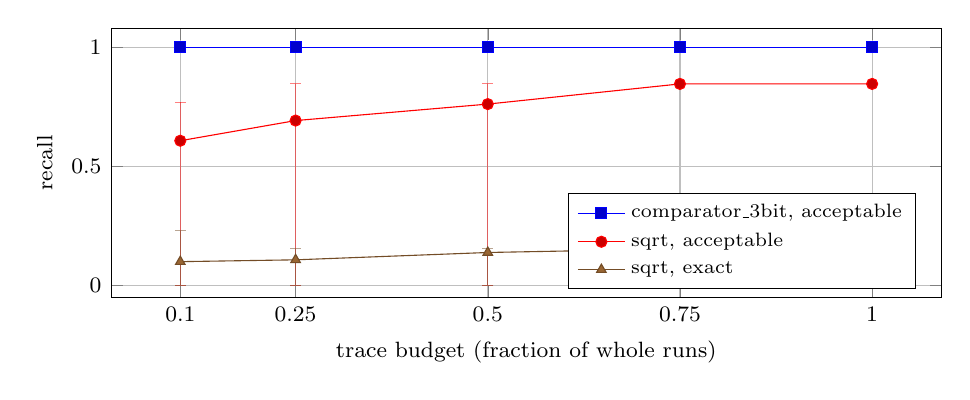
\begin{tikzpicture}
\begin{axis}[width=\columnwidth,height=5cm,
  xlabel={trace budget (fraction of whole runs)}, ylabel={recall},
  xtick={0.1,0.25,0.5,0.75,1.0}, ymin=-0.05, ymax=1.08,
  legend pos=south east, legend style={font=\scriptsize,cells={anchor=west}},
  grid=major, font=\footnotesize,
  error bars/error bar style={opacity=0.5}]
% tools/report_rqs.py --section rq3 ; bars are min/max over 10 seeds
\addplot+[mark=square*,error bars/.cd,y dir=both,y explicit] coordinates {
(0.10,1.0000) += (0,0.0000) -= (0,0.0000) (0.25,1.0000) += (0,0.0000) -= (0,0.0000) (0.50,1.0000) += (0,0.0000) -= (0,0.0000) (0.75,1.0000) += (0,0.0000) -= (0,0.0000) (1.00,1.0000) += (0,0.0000) -= (0,0.0000)
};
\addlegendentry{comparator\_3bit, acceptable}
\addplot+[mark=*,error bars/.cd,y dir=both,y explicit] coordinates {
(0.10,0.6077) += (0,0.1615) -= (0,0.6077) (0.25,0.6923) += (0,0.1538) -= (0,0.6923) (0.50,0.7615) += (0,0.0846) -= (0,0.7615) (0.75,0.8462) += (0,0.0000) -= (0,0.0000) (1.00,0.8462) += (0,0.0000) -= (0,0.0000)
};
\addlegendentry{sqrt, acceptable}
\addplot+[mark=triangle*,error bars/.cd,y dir=both,y explicit] coordinates {
(0.10,0.1000) += (0,0.1308) -= (0,0.1000) (0.25,0.1077) += (0,0.0462) -= (0,0.1077) (0.50,0.1385) += (0,0.0154) -= (0,0.1385) (0.75,0.1538) += (0,0.0000) -= (0,0.0000) (1.00,0.1538) += (0,0.0000) -= (0,0.0000)
};
\addlegendentry{sqrt, exact}
\end{axis}
\end{tikzpicture}
\caption{RQ3. Guarantee recall against trace budget, mean over ten seeds, bars to the worst
and best seed. \texttt{sqrt} saturates at 75\% of its corpus; the downward bars at the small
budgets are the seeds for which no trigger beat its null model and the flow returned no
region at all.}
\label{fig:budget}
\end{figure}

\subsection{RQ4: how much grammar is worth paying for}
\label{sec:rq4}
The template grammar is the one configuration knob that decides what shape of property can be
expressed at all, and \ACE{} ships five nested vocabularies \Grammar{} from a single
implication to a five-template set with conjunctive antecedents and a sequence
antecedent.\footnote{\texttt{ace/backends.py:56--72}. \texttt{G1}$\subset\cdots\subset$\texttt{G5}.}
Each design was mined under each, everything else fixed, with a budget of 1800\,s per point
after which the point is recorded as incomplete rather than allowed to stall the
sweep.\footnote{\texttt{tools/sweep.py}, \texttt{--timeout}.} Table~\ref{tab:rq4} is the
result, and the first thing it says is not about recall. \emph{Eight of the eleven designs do
not complete under \texttt{G4} or \texttt{G5} at all.} Only \texttt{adder\_8bit},
\texttt{comparator\_3bit} and \texttt{ibex\_csr} --- the three smallest --- finish under every
grammar. Averaging each grammar over whatever finished would score \texttt{G5} on an easier
benchmark than \texttt{G1} and reward a grammar for failing, so the means in
Table~\ref{tab:rq4} are over those three; the per-design rows below them carry the rest.

What the wide grammars cost is visible even on the three that survive: \texttt{G4} and
\texttt{G5} take 390\,s and 503\,s against \texttt{G3}'s 25\,s, a factor of 16 to 20, for
clause volumes three and five times larger. Neither buys anything on those designs ---
\texttt{G4} matches \texttt{G3} exactly and \texttt{G5} is \emph{worse} (92\% against 100\%
acceptable, 45\% against 57\% exact), because a larger grammar finds more ways to state the
same obligation and a reference matched exactly under a smaller one can end up matched by a
refinement instead.

The useful range is therefore \texttt{G1} to \texttt{G3}, where every design completes.
Across all eleven, mean acceptable recall goes 51\%, 76\%, 82\% and mean exact recall 26\%,
39\%, 43\%, for 18\,s, 22\,s and 25\,s on the three-design common set. The step from
\texttt{G1} to \texttt{G2} --- adding the next-cycle implication $G(P_0\mid\Rightarrow P_1)$
--- is the one that matters, and it is nearly free. \texttt{G3}'s bounded window then buys six
further points and is the default. The gain is concentrated rather than general:
\texttt{apb\_slave} goes from 6\% to 94\% and \texttt{sqrt} from 23\% to 85\% across that
range, while \texttt{ibex\_alu}, \texttt{adder\_8bit} and \texttt{comparator\_3bit} do not
move at all.

\begin{table}[t]
\centering
\caption{RQ4. Grammar against what it recovers and what it costs. \emph{designs} is how many
of the eleven completed within 1800\,s per point; means, clause counts and seconds are over
the three that completed under every grammar. Recalls are percentages; seconds are the sum of
the per-design wall clock.}
\label{tab:rq4}
\begin{tabular}{lrrrrrrr}
\toprule
& designs & exact & acc & mined & distinct & s & peak MiB \\
\midrule
% tools/report_rqs.py --section rq4
G1 & 11/11 & 49 & 75 & 179 & 167 & 18 & 47 \\
G2 & 11/11 & 57 & 100 & 299 & 274 & 22 & 58 \\
G3 & 11/11 & 57 & 100 & 400 & 373 & 25 & 66 \\
G4 & 3/11 & 57 & 100 & 1368 & 1144 & 390 & 148 \\
G5 & 3/11 & 45 & 92 & 1849 & 1529 & 503 & 191 \\
\midrule
\multicolumn{8}{l}{\emph{acceptable recall per design}} \\
ibex\_alu & 72 & 72 & 72 & -- & -- & & \\
ibex\_csr & 25 & 100 & 100 & 100 & 75 & & \\
ibex\_multdiv\_fast & 54 & 54 & 69 & -- & -- & & \\
apb\_slave & 6 & 67 & 94 & -- & -- & & \\
arbiter4 & 28 & 50 & 50 & -- & -- & & \\
fifo\_sync & 33 & 67 & 67 & -- & -- & & \\
accumulator & 40 & 60 & 60 & -- & -- & & \\
adder\_8bit & 100 & 100 & 100 & 100 & 100 & & \\
comparator\_3bit & 100 & 100 & 100 & 100 & 100 & & \\
multi\_16bit & 75 & 100 & 100 & -- & -- & & \\
sqrt & 23 & 62 & 85 & -- & -- & & \\
\bottomrule
\end{tabular}
\end{table}

\subsection{RQ5: what the flow costs}
\label{sec:rq5}
Cost was measured with the flow run one design at a time on an otherwise idle machine, at
each design's own grammar, with per-stage wall clock taken by the flow itself and peak
resident set read from the process that hosts the miner.\footnote{\texttt{ace/\_\_main\_\_.py:29--35};
\texttt{tools/sweep.py}, \texttt{resource.RUSAGE\_CHILDREN}.} Table~\ref{tab:rq5} reports it.

The headline is what is \emph{absent}. No stage of the flow invokes a simulator: events are
labelled by one linear scan of the traces, episodes are clipped from them, and the IP is
never encapsulated, forced or re-run. Simulation time does not appear in Table~\ref{tab:rq5}
because it is not merely reduced but structurally gone, and with it the dependence on owning
a simulator licence and a synthesisable wrapper for the IP.

What remains is the miner. Mining is 76--100\% of every run and at least 92\% on ten of the
eleven designs; every other stage together --- loading, labelling, trigger selection, episode
extraction, cross-event merging --- costs at most 3.3\,s on every design, and under a second
on seven of them. Absolute cost at this scale: the whole eleven-design benchmark is 2176\,s
serial and the largest single run is 909\,s, at a peak of 385\,MiB.

Neither runtime nor memory tracks trace length. \texttt{accumulator} is 19000 samples and
costs 35\,s; \texttt{ibex\_multdiv\_fast} is 7500 and costs 909\,s. What they track is the
volume the miner is handed and the width of the vocabulary over it: the divider's single
region keeps 7491 of its 7500 samples, so decomposition removes almost nothing and the miner
sees essentially the full corpus with an eight-signal interface, while the accumulator's
region is 5788 of 19000. Episode extraction is therefore the flow's real cost control, and it
pays exactly when the behavior being separated is sparse in the trace. The horizon compounds
it: a bounded-response clause is re-offered at every fixed latency inside its window, so the
post-mining pass over the clause set grows with $H$ as well as with the set, which is why the
two designs with the widest windows --- \texttt{ibex\_multdiv\_fast} at $H=40$ and
\texttt{sqrt} at $H=24$ --- are the two most expensive runs in the table.
Grammar dominates both, and more sharply than either: across \texttt{G1}--\texttt{G5} the
three designs that complete under every grammar span 18\,s to 503\,s, and eight of the eleven
do not complete under the two widest grammars at all (Table~\ref{tab:rq4}). That is a
configuration choice, not a property of the traces.

\begin{table}[t]
\centering
\caption{RQ5. Cost per design at its own grammar, measured serially. \emph{sig} is interface
signals, \emph{ep.\ samples} the samples the miner is handed, summed over regions --- it
exceeds the corpus where two regions overlap, as on \texttt{arbiter4},
\emph{mine} the share of wall clock inside the miner.}
\label{tab:rq5}
\begin{tabular}{lrrrrrrr}
\toprule
design & samples & sig & ep.\ samples & mine s & total s & mine \% & MiB \\
\midrule
% tools/report_rqs.py --section rq5
ibex\_alu & 6000 & 6 & 3661 & 36.6 & 38.7 & 95 & 62 \\
ibex\_csr & 2500 & 5 & 548 & 3.9 & 4.2 & 92 & 56 \\
ibex\_multdiv\_fast & 7500 & 8 & 7491 & 908.6 & 909.1 & 100 & 259 \\
apb\_slave & 6000 & 9 & 6081 & 148.0 & 156.8 & 94 & 181 \\
arbiter4 & 5000 & 11 & 8360 & 142.7 & 143.6 & 99 & 168 \\
fifo\_sync & 6000 & 8 & 4032 & 92.5 & 93.3 & 99 & 127 \\
accumulator & 19000 & 5 & 5788 & 33.8 & 34.8 & 97 & 287 \\
adder\_8bit & 2500 & 5 & 1709 & 3.1 & 3.3 & 94 & 47 \\
comparator\_3bit & 2000 & 5 & 1892 & 1.4 & 1.8 & 76 & 36 \\
multi\_16bit & 5000 & 6 & 4950 & 274.9 & 275.3 & 100 & 189 \\
sqrt & 20000 & 6 & 16553 & 511.3 & 514.6 & 99 & 385 \\
\bottomrule
\end{tabular}
\end{table}

\subsection{Threats to validity}
\label{sec:threats}
\emph{Every category is trace-bounded.} Equivalence, refinement and subsumption are decided
by evaluating clauses over the observed corpus, so a mined clause reported equivalent to a
reference clause agrees with it on the traces at hand and is not proved equal to it. Two
clauses that differ only where the stimulus never went are indistinguishable here. Replacing
the evaluator with an SMT or model-checking backend in Step~5 would turn these categories into
proofs, and is the largest single gap between the implementation and the method it
implements.\footnote{\texttt{reports/METHODOLOGY\_COMPATIBILITY.md}, Step~5.}

\emph{The declared part of the vocabulary was written from the reference set.} Every number
here measures the flow given a good vocabulary, which is the fair way to read
Table~\ref{tab:rq2} and an unfair way to read it as a prediction for an undocumented IP. The
conjunctions, relations and transitions \ACE{} adds to it are derived from the traces and see
nothing of the reference set, so they do not widen that threat; the hand-written propositions
they are built from do. How much recall survives a vocabulary derived from the interface alone
is a question about the miner rather than about the decomposition, and is not evaluated here.

\emph{Recall is reported, precision is not.} The mined guarantee set is two orders of
magnitude larger than the reference set, and no trace-side signal we measured separates the
two: ranking by support, by delay tightness, by antecedent size or by interface relevance
leaves the reference-matching clauses at ranks in the hundreds, so a reported top-$k$ would
cost recall rather than buy precision. Nor are the extras weak consequences to fold away ---
none is implied by a reference contract, they survive the stress corpus and they generalize
to the held-out runs. Separating them needs a criterion from outside the traces, such as
mutation-based importance or engineer triage of a ranked list, which is why the artifact
reports the extras per design rather than hiding them behind a recall
percentage.\footnote{\texttt{RECOVERY.md}, \emph{Precision}; per-design counts in
\texttt{CONTRACT\_RECOVERY.md}.}

\emph{The reference sets are hand-encoded and finite.} A missed clause is a clause the flow
did not recover from these traces; it is not evidence that the IP violates it, and a recovered
clause is not evidence that the reference set is complete. Recall is computed against what was
written down, so a behavior nobody documented cannot be missed. One consequence bounds
\S\ref{sec:rq1} specifically. Every reference guarantee was validated to hold over the whole
corpus, so the reference set contains no region-local obligation and the coverage comparison
cannot score the clauses decomposition uniquely reaches; its guarantee-side result is a
no-loss bound rather than an upper bound on what decomposition can do. That those clauses are
beyond the control is measured separately and does not depend on the reference set
(\S\ref{sec:rq1}), but their \emph{worth} is not established by anything here: on this
benchmark they are artifacts of how regions are anchored and of the range the stimulus swept.
What is missing is therefore not expressive power, which the measurement shows decomposition
has, but a stimulus that makes region-local clauses obligations rather than sampled ranges,
together with a reference set that contains them so they can be scored.

\emph{Scale.} The corpus is eleven blocks of between 2000 and 20000 samples and between five
and twelve interface signals. The Ibex designs are sub-blocks of a production core, not the
core; no SoC-scale IP is included, so \S\ref{sec:rq5} shows how cost grows with trace length
and interface width over that range and not that the flow holds at an order of magnitude
beyond it.

\emph{Compositional use is not evaluated.} Mining a producer and a consumer independently and
discharging the producer's guarantee against the consumer's assumption is the use case that
motivates A/G contracts, and checking that discharge needs a formal engine rather than a
trace evaluator. It is left as future work, for the same reason as the SMT backend above.
